\documentclass[12pt,a4paper]{report}
\usepackage[portuguese]{babel}
\usepackage[utf8]{inputenc}
\usepackage{array}
\usepackage{xcolor}
\usepackage{graphicx}
\usepackage{float} 
\usepackage[pdftex]{hyperref}
\usepackage{titling}
\usepackage{amsmath}
\usepackage{booktabs}
\setlength{\parindent}{0pt}

\setlength{\droptitle}{-2cm}

\title{Projeto de Processamento de Linguagens 2025\\[1em]
            \textbf{Construção de um Compilador para Pascal Standard}
            \\[1em]Relatório Técnico
        }
\author{
    Grupo 12 - Equipa Bugbusters \raisebox{-0.5ex}{
\includegraphics[width=1em]{cover/Beetle_Emoji.png}
\includegraphics[width=1em]{cover/Prohibited_Emoji.png}}\\\\
    \begin{tabular}{ccc}
    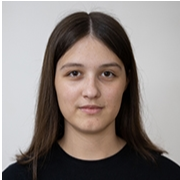
\includegraphics[width=3.5cm, height=3.5cm]{cover/A104437.png} & 
\includegraphics[width=3.5cm, height=3.5cm]{cover/A104263.png} & 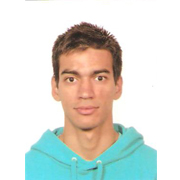
\includegraphics[width=3.5cm, height=3.5cm]{cover/A76350.jpg} \\
    Ana Sá Oliveira & Inês Silva Marques & José Rafael de \\
    (a104437) & (a104263) & Oliveira Vilas Boas \\
    && (a76350) \\
    \end{tabular}
    \\
    
\includegraphics[width=4cm, height=4cm]{cover/Bugbusters.png}
    \\
}
\date{\today}

\begin{document}
\maketitle
\begin{abstract}
    Este projeto teve como objetivo o desenvolvimento de um compilador para a linguagem Pascal Standard. O compilador foi construído em várias etapas, começando pela análise léxica, utilizando a biblioteca ply.lex para transformar o código-fonte em uma sequência de tokens. A seguir, foi implementada a análise sintática com ply.yacc, validando a estrutura do programa com base na gramática da linguagem.
    A partir do código reconhecido, foi construída uma árvore sintática abstrata (AST), que representa de forma estruturada os elementos do programa. Com base nessa AST, foi realizada a análise semântica, incluindo verificação de tipos de dados, declarações de variáveis e coerência do código.
    Na etapa de geração de código, a AST foi transformada diretamente em código para a máquina virtual do projeto. Para cada etapa, foram realizados testes automáticos com os exemplos de código Pascal fornecidos no enunciado.
\end{abstract}

\tableofcontents
%\listoffigures
%\listoftables

\chapter{Introdução}
%\section{}
%\subsection{}
O objetivo deste projeto foi desenvolver um compilador para a linguagem Pascal standard. Mais concretamente,
pretendeu-se implementar um compilador capaz de analisar, interpretar e traduzir código Pascal para um formato
intermediário e deste para código máquina ou diretamente para código máquina, neste caso da VM
disponibilizada aos alunos. A equipa optou por primeiro passar o código Pascal para um formato intermediário e só depois passar deste para código máquina.
O compilador deve ser capaz de processar programas Pascal standard, incluindo declaração de variáveis,
expressões aritméticas e comandos de controle de fluxo (if, while, for), e, opcionalmente, subprogramas
(procedure e function).

\vspace{1em}

Para construir este compilador, tivemos várias etapas:
\begin{enumerate}
    \item Análise léxica;
    \item Análise sintática;
    \item Árvore sintática abstrata (AST);
    \item Análise semântica;
    \item Geração de código.
\end{enumerate}

Para além dessas etapas, foi também necessário realizar testes, os quais foram conduzidos de forma contínua ao longo do desenvolvimento.

\chapter{Análise Léxica}

A análise léxica consistiu em implementar um analisador léxico (lexer) para converter código Pascal numa lista de tokens. Para implementar este lexer,
usamos a ferramenta ply.lex, já conhecida das aulas.

\section{Palavras Reservadas}

O primeiro passo foi identificar as palavras reservadas da linguagem Pascal standart.

\begin{center}
\begin{tabular}{>{\ttfamily} l >{\ttfamily} l >{\ttfamily} l >{\ttfamily} l}
\toprule
and & array & begin & case \\
const & div & do & downto \\
else & end & file & for \\
function & goto & if & in \\
label & mod & nil & not \\
of & or & packed & procedure \\
program & record & repeat & set \\
then & to & type & until \\
var & while & with & \\
\bottomrule
\end{tabular}
\end{center}

Cada palavra reservada resulta num token que definimos.

\vspace{1em}

Por exemplo, o token BEGIN (palavra reservada begin) definimos da seguinte forma:

\begin{verbatim}
def t_BEGIN(t):
    r'[bB][eE][gG][iI][nN]\b'
    return t
\end{verbatim}

Nesta expressão regular, cada letra aparece entre colchetes com as duas versões maiúscula e minúscula, o que permite que o reconhecimento seja \emph{case insensitive}, aceitando \texttt{begin}, \texttt{Begin}, \texttt{BEGIN}, etc.

O símbolo \texttt{\\b} representa uma \emph{boundary} (limite de palavra), garantindo que o lexer reconheça apenas a palavra completa \texttt{begin} e não uma parte de outra palavra maior, como \texttt{beginning}

\section{Literals}

O segundo passo foi identificar os simbolos únicos, os literals, compostos apenas por um caracter, desta linguagem.

\begin{center}
\begin{tabular}{>{\ttfamily} l >{\ttfamily} l >{\ttfamily} l >{\ttfamily} l}
\toprule
+ & - & * & / \\
= & < & > & [ \\
] & . & , & : \\
; & \^{} & ( & ) \\
\bottomrule
\end{tabular}
\end{center}

Cada um destes simbolos é um token.

\section{Restantes tokens}

O terceiro passo foi identificar os restantes tokens:
\begin{center}
\begin{tabular}{>{\ttfamily} l >{\ttfamily} l >{\ttfamily} l >{\ttfamily} l}
\toprule
NOT\_EQUAL & LESS\_EQUAL & GREATER\_EQUAL & ASSIGNMENT \\
RANGE & LPA & ARP & LPP \\
PRP & BOOL & DATATYPE & ID \\
INT & REAL & STRING & COMMENT \\
\bottomrule
\end{tabular}
\end{center}

Os tokens do analisador léxico incluem operadores relacionais como o \texttt{NOT\_EQUAL}, que representa o símbolo de diferente (\texttt{<>}), além do \texttt{LESS\_EQUAL} e \texttt{GREATER\_EQUAL}, correspondentes aos operadores “menor ou igual” (\texttt{<=}) e “maior ou igual” (\texttt{>=}), respectivamente. O token \texttt{ASSIGNMENT} identifica o operador de atribuição usado em Pascal, que é representado por \texttt{:=}. Para representar intervalos, utiliza-se o token \texttt{RANGE}, que corresponde ao símbolo \texttt{..}.

O token \texttt{BOOL} é usado para valores booleanos, como \texttt{true} e \texttt{false}, e o \texttt{DATATYPE} identifica os tipos de dados básicos da linguagem, incluindo \texttt{integer}, \texttt{real}, \texttt{char}, entre outros. Para nomes de variáveis, funções e procedimentos, o token \texttt{ID} é responsável por reconhecer os identificadores.

Números inteiros e reais são capturados pelos tokens \texttt{INT} e \texttt{REAL}, respectivamente, enquanto cadeias de caracteres delimitadas por aspas são reconhecidas pelo token \texttt{STRING}. Por fim, o token \texttt{COMMENT} é utilizado para identificar os comentários no código, que são ignorados durante a compilação.

Quanto a símbolos delimitadores, temos os tokens \texttt{LPA} e \texttt{ARP}, que correspondem a\texttt{(*} e \texttt{*)}, respectivamente, enquanto \texttt{LPP} e \texttt{PRP} representam \texttt{[} e \texttt{]}.

Assim, o analisador léxico, o \texttt{pascal\_analex.py}, transforma o código pascal numa sequência de tokens. Se existir algum caracter ilegal, o lexer irá mostrar onde ocorreu o erro.

\chapter{Análise Sintática}

A análise sintática consistiu em construir um analisador sintático (parser) para validar a estrutura gramatical do código. Para implementar o parser usamos a ferramenta ply.yacc.

\section{Gramática}
O primeiro passo consiste em definir uma gramática da linguagem:

\begin{tabbing}
\hspace{1.3cm}\= \hspace{11cm}\= \kill
\textbf{p0:}  \> S' \(\to\) program \\
\textbf{p1:}  \> program \(\to\) PROGRAM ID ; declarations code\_block . \\
\textbf{p2:}  \> program \(\to\) declarations code\_block . \\
\textbf{p3:}  \> declarations \(\to\) declarations declaration \\
\textbf{p4:}  \> declarations \(\to\) \(\epsilon\) \\
\textbf{p5:}  \> declaration \(\to\) variables\_declaration \\
\textbf{p6:}  \> declaration \(\to\) function \\
\textbf{p7:}  \> declaration \(\to\) procedure \\
\textbf{p8:}  \> variables\_declaration \(\to\) VAR variables\_list \\
\textbf{p9:}  \> variables\_list \(\to\) variables\_list same\_type\_variables \\
\textbf{p10:} \> variables\_list \(\to\) same\_type\_variables \\
\textbf{p11:} \> same\_type\_variables \(\to\) id\_list : DATATYPE ; \\
\textbf{p12:} \> same\_type\_variables \(\to\) id\_list : ARRAY [ INT RANGE INT ] OF DATATYPE ; \\
\textbf{p13:} \> id\_list \(\to\) id\_list , ID \\
\textbf{p14:} \> id\_list \(\to\) ID \\
\textbf{p15:} \> var\_or\_not \(\to\) variables\_declaration \\
\textbf{p16:} \> var\_or\_not \(\to\) \(\epsilon\) \\
\textbf{p17:} \> function \(\to\) FUNCTION ID ( parameters ) : DATATYPE ; var\_or\_not code\_block ; \\
\textbf{p18:} \> procedure \(\to\) PROCEDURE ID ( parameters ) ; var\_or\_not code\_block ; \\
\textbf{p19:} \> parameters \(\to\) parameter\_list \\
\textbf{p20:} \> parameters \(\to\) \(\epsilon\) \\
\textbf{p21:} \> parameter\_list \(\to\) parameter\_list ; parameter \\
\textbf{p22:} \> parameter\_list \(\to\) parameter \\
\textbf{p23:} \> parameter \(\to\) VAR\_opt id\_list : DATATYPE \\
\textbf{p24:} \> VAR\_opt \(\to\) VAR \\
\textbf{p25:} \> VAR\_opt \(\to\) \(\epsilon\) \\
\textbf{p26:} \> code\_block \(\to\) BEGIN algorithm END \\
\textbf{p27:} \> algorithm \(\to\) algorithm ; statement \\
\textbf{p28:} \> algorithm \(\to\) statement \\
\textbf{p29:} \> statement \(\to\) assignment \\
\textbf{p30:} \> statement \(\to\) func\_call \\
\textbf{p31:} \> statement \(\to\) loop \\
\textbf{p32:} \> statement \(\to\) code\_block \\
\textbf{p33:} \> statement \(\to\) if \\
\textbf{p34:} \> statement \(\to\) else \\
\textbf{p35:} \> statement \(\to\) \(\epsilon\) \\
\textbf{p36:} \> if \(\to\) IF cond THEN statement \\
\textbf{p37:} \> else \(\to\) IF cond THEN statement ELSE statement \\
\textbf{p38:} \> assignment \(\to\) ID ASSIGNMENT cond \\
\textbf{p39:} \> loop \(\to\) for \\
\textbf{p40:} \> loop \(\to\) while \\
\textbf{p41:} \> for \(\to\) FOR for\_cond DO statement \\
\textbf{p42:} \> for\_cond \(\to\) assignment TO cond \\
\textbf{p43:} \> for\_cond \(\to\) assignment DOWNTO cond \\
\textbf{p44:} \> while \(\to\) WHILE cond DO statement \\
\textbf{p45:} \> cond \(\to\) expr \\
\textbf{p46:} \> cond \(\to\) expr op\_rel expr \\
\textbf{p47:} \> op\_rel \(\to\) = \\
\textbf{p48:} \> op\_rel \(\to\) NOT\_EQUAL \\
\textbf{p49:} \> op\_rel \(\to\) < \\
\textbf{p50:} \> op\_rel \(\to\) LESS\_EQUAL \\
\textbf{p51:} \> op\_rel \(\to\) > \\
\textbf{p52:} \> op\_rel \(\to\) GREATER\_EQUAL \\
\textbf{p53:} \> expr \(\to\) termo \\
\textbf{p54:} \> expr \(\to\) expr op\_ad termo \\
\textbf{p55:} \> termo \(\to\) fator \\
\textbf{p56:} \> termo \(\to\) termo op\_mul fator \\
\textbf{p57:} \> op\_ad \(\to\) + \\
\textbf{p58:} \> op\_ad \(\to\) - \\
\textbf{p59:} \> op\_ad \(\to\) OR \\
\textbf{p60:} \> op\_mul \(\to\) * \\
\textbf{p61:} \> op\_mul \(\to\) / \\
\textbf{p62:} \> op\_mul \(\to\) AND \\
\textbf{p63:} \> op\_mul \(\to\) MOD \\
\textbf{p64:} \> op\_mul \(\to\) DIV \\
\textbf{p65:} \> fator \(\to\) value \\
\textbf{p66:} \> fator \(\to\) ( cond ) \\
\textbf{p67:} \> fator \(\to\) NOT fator \\
\textbf{p68:} \> value \(\to\) ID \\
\textbf{p69:} \> value \(\to\) INT \\
\textbf{p70:} \> value \(\to\) REAL \\
\textbf{p71:} \> value \(\to\) STRING \\
\textbf{p72:} \> value \(\to\) BOOL \\
\textbf{p73:} \> value \(\to\) ID [ INT ] \\
\textbf{p74:} \> value \(\to\) ID [ ID ] \\
\textbf{p75:} \> value \(\to\) func\_call \\
\textbf{p76:} \> func\_call \(\to\) ID ( args ) \\
\textbf{p77:} \> args \(\to\) elems \\
\textbf{p78:} \> args \(\to\) \(\epsilon\) \\
\textbf{p79:} \> elems \(\to\) elems , cond \\
\textbf{p80:} \> elems \(\to\) cond \\
\end{tabbing}

\textcolor{red}{\textbf{TODO}}

\chapter{Árvore Sintática Abstrata (AST)}

\textcolor{red}{\textbf{TODO}}

\chapter{Análise Semântica}

A análise semântica consistiu em verificar tipos de dados, declaração de variáveis e coerência do código. Para o fazer, percorremos a AST e fomos guardando algumas informações
e verificando outras.

Em concreto, na análise semântica:
\begin{enumerate}
    \item não permitimos que se use variáveis que não tenham sido declaradas antes (dá erro);
    \item verificamos quando se atribui uma variável a uma expressão, que ambas teem o mesmo tipo;
    \item verificamos o tipo dos operadores numa operação e vemos se são os adequados.
    \item ...
\end{enumerate}

\chapter{Geração de Código}

\textcolor{red}{\textbf{TODO}}

\chapter{Testes}

Ao longo do desenvolvimento do projeto foram realizados testes.

Tanto o analisador léxico, como analisador sintático, semantico como o compilador teem modo interativo, onde podemos testar código pascal.

Mas ainda fizemos o \texttt{pascal\_test.py} que faz a analise léxica, sintática, semântica e gera código e valida ese mesmo código, isto tudo sobre os códigos em Pascal usados como exemplo no
enunciado do projeto.

Havia 7 códigos em Pascal no enunciado. Todos os códigos passam os testes de analise léxica, sintática e semântica porque são programas corretos, sem erros léxicos, sintáticos ou semanticos.
Código de máquina é gerado para os 7 exemplos. E por fim, validamos o código de máquina gerado. Os exemplos 1 a 6 teem código gerado correto. O único código gerado errado é o do exemplo 7, porque já leva
em conta as funções, um extra que não implementámos na analise semântica nem a gerar código.

\begin{figure}[H]
    \centering
    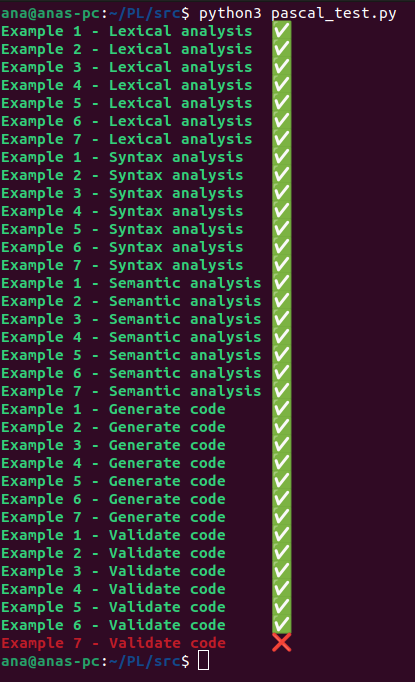
\includegraphics[width=8cm]{images/tests.png}
    \caption{Testes automáticos.}    
\end{figure}

\chapter{Conclusão}

Concluindo, conseguimos alcançar o objetivo principal deste projeto: construir um compilador para a linguagem Pascal Standard, que transforme código Pascal em código da máquina virtual.
O nosso compilador é capaz de processar programas Pascal standart com declarações de variáveis, expressões aritméticas e comandos de controle de fluxo (if, while, for). Para além disto,
seguimos as etapas do projeto: construímos um analisador léxico, um analisador sintático, fizemos uma árvore sintática abstrata, fizemos um analisador semântico, geramos o código desejado
e ainda fizemos testes de tudo isto, para garantir a correção de todos estes programas.

\vspace{1em}

Assim, concluímos que conseguimos cumprir os principais objetivos do projeto. Ficou por fazer alguns extras como otimizações do código máquina e suporte a subprogramas (functions e procedures).
Estes subprogramas estão suportados até ao nosso analisador sintático inclusive, mas depois não os implementamos nas fases seguintes.

\end{document}